In this section, we will focus on the analysis of different databases based on the  evaluation of XMark queries. BaseX, Mongodb, Couchbase and RethinkDB are  completely different database system  with their own data model and different query languages. Even all the NoSQL databases have different structures and query model.  Due to their complete different nature, a query of a database would perform better than others if data was normalized according their specified data model then our requirements. For example, BaseX would probably perform better if the data was normalized as well. Therefore, our goal is not to compare queries between theses databases but evaluates the results individually.  Each databases has been tested in 6 different size XMark data as mentioned in ~\ref{xmark}. Firstly, we will analyze result of each of the four systems. Finally, we will check the all database together in a single figure for 111MB dataset. 

\subsection{MongoDB}
Figure~\ref{fig:xmark-result-mongodb-all} presents the time measurement of XMark queries in MongoDB. MongoDB automatically uses all the free memory of a machine for its cache. But this usage is dynamic and if other processes need the Server's RAM, it handover such cached memory to other process. Hence, the result of XMark queries might depends on the other processes running in the machine.  The result of the queries will be explained below:
\begin{itemize}
\item The simplest query Q1 was the most efficient query for all instances of database and executed less than 4ms. Conditional operator on the default index \textit{\_id} made it faster.
\item Q3 and Q4 were relatevely slower queries due to multi-stage array processing with aggregation pipeline. Even two secondary indexes were used, the performance of these queries could not be competitive to other systems. 
\item The \textit{count} operation in MongoDB with simple filtration is comparatively faster than other NoSQL databases, Q5 and Q6 are used to count the number of documents in a collection with criteria. In Q5, the secondary index in field \textit{price}  helped to accelerate the performance. Figure~\ref{fig:xmark-mongodb-index-noindex} clarifies the efficiency of two queries Q5 and Q13 where the execution time improved exponentially after the indexes. In Q6, just the \textit{count()} operation in a collection due to data model defined in ~\ref{xmark-mongodb} made better performance possible. 

\item Among the join queries, Q8 and Q9 generated the best result in case of execution time among the other system, once again the indexes created in these two queries improved the performance. But in case of Q10, complex result generations with joins could not be completed for two databases, a large output with many new fields made the query inefficient. The value join queries in Q11 and Q12 has to deal with many read operations due to manual join, therefore these queries also did not perform well.

\item The secondary index in Q13 helped to keep execution time low, As mentioned earlier the Fig.~\ref{fig:xmark-result-mongodb-13} shows the time consumed by Q13  with and without index. Q14 is used to search for sub-string instead of full text search of XQuery, the relative performance was decreased when the size of database in increased.

\item The structures of the queries in Q15 and Q16 are complex in all NoSQL databases including MongoDB because of deep path in XQuery and has to process many array and object elements. The results produced in these queries were not exactly same as of XQuery but the performance was in the same level and the size of database did not have greater effect. The result of Q17 was similar to that of other systems but performance of Q18 has been decreased when database get bigger. 
Q19 returned result in new field \textit{item} that reduces the performance because  MongoDB has to use aggregation pipeline for new field.  The Query would be much more faster if the result would be return without new element using \textit{find} function. 
\item Finally, the query Q20 groups, categories them and returns cardinalities. As the database get bigger query became slower. 
\end{itemize}
\begin{figure}
	\centering
	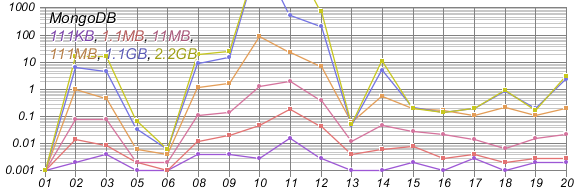
\includegraphics[width=0.95\textwidth]{img/result/mongodb/mongodb-all}
	\caption{XMark queries in MongoDB}
	\label{fig:xmark-result-mongodb-all}
	
\end{figure}	
\begin{figure}
	\centering
	\subfloat[Q5]{
		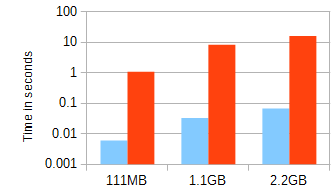
\includegraphics[width=0.4\textwidth]{img/result/mongodb/mongodb-q5-index-noindex}
		\label{fig:xmark-result-mongodb-5}
	}
	\centering
	\subfloat[Q13]{
		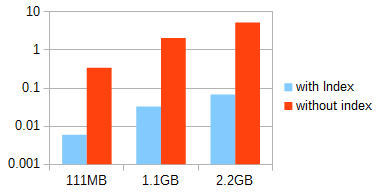
\includegraphics[width=0.4\textwidth]{img/result/mongodb/mongodb-q13-index-noindex}
		\label{fig:xmark-result-mongodb-13}
	}
	\caption{MongoDB queries with and without secondary index in different database instances}
	\label{fig:xmark-mongodb-index-noindex}
\end{figure}

\subsection{Basex}
The results of all six different databases in BaseX is shown in figure~\ref{fig:xmark-result-basex-all}. All the queries were tested with text, attribute and full text indexes. The query Q1 utilize the attributes index and return result a single result. This query was completed in less than 5mm in all databases. The query Q2 and Q3  with positional predicates took longer time if the the size of database is increases. The queries Q5 and Q6 uses count operation and both were relatively faster. As we've seen previous section, these queries performed better in MongoDB than in BaseX. Among the join-queries,  Q11 and Q12 could not be completed in defined time frame for databases bigger than 11MB. For reference join on attributes values defined in Q8 and Q9, the attribute index is utilized to get result. The time taken by these two queries is  similar to that of MongoDB.  The full text search query Q14 was slightly affected by the size of database. The queries Q15-Q17 implements the location paths, with similar performances and query Q18  implements user defined function for calculation. Q19 consumes most of resources for sorting for data. This query is faster in Mongodb compare to BaseX. Finally, the aggregation query Q20 produces constant result in all databases instances. 
\begin{figure}
	\centering
	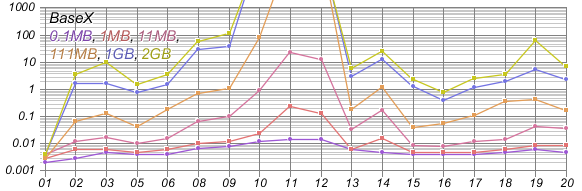
\includegraphics[width=0.95\textwidth]{img/result/basex/basex-all}
	\caption{XMark queries in BaseX}
	\label{fig:xmark-result-basex-all}
\end{figure}

\subsection{RethinkDB}
All the time evaluation of XMark queries in RethinkDB is given in Fig.~\ref{fig:xmark-result-rethinkdb-all}. 
\begin{itemize}
\item Query Q1 is consume more time compare to MongoDB and BaseX in average.
 \item  
  RethinkDB is able to handle arrays better ways than other NoSQL databases. Chains of queries can be used as a pipeline but unlike MongoDB's pipeline that produces result in multiple stages, RethinkDB runs a query on a server and once, hence it has been seen that queries Q2 and Q3 produces better result compare to MongoDB. 
 \item
 Queries Q5 and Q6 were comparatively slow in  RethinkDB. Firstly, MongoDB uses secondary index on Q5, but RethinkDB cannot be used a index in \textit{filter()} function. Secondly, the \textit{count()} operation in RethinkDB is always slow due to stream properties. It executes everything in server, most of the stream operations \todo{explain stream/lazy operation in introduction} including \textit{filter} runs lazily. The \textit{run} functions returns the results as soon as the first block of data is available, it does not load whole table data  at once. It will load rest of data as clients iterate over the cursor, therefore it does not keep much memory at once. In case of \textit{count()}, the query has to wait until all the data is loaded. 
 \item As we have mentioned the support of join query in ~\ref{xmark-rethinkdb}, RethinkDB was not able to take advantages of native joins except query Q11 and Q12. The join operation in Q8, Q9 and Q10 were similar in case of time measurement with rest of system. Q10 is slower due to large output and many new fields. 
 \item In query Q13, index is utilized on \textit{regions} field of the table that produces comparable result to MongoDB but better than BaseX. Queries Q14-Q19 are returned similar result except in Q15, due to many array sand object operations. 
\item The query Q20 was once again slow in RethinkDB due to cardinalities at the end of the query. All the grouping and categorizing operations were a lot faster than counting at the end. 
\end{itemize}

\begin{figure}
	\centering
	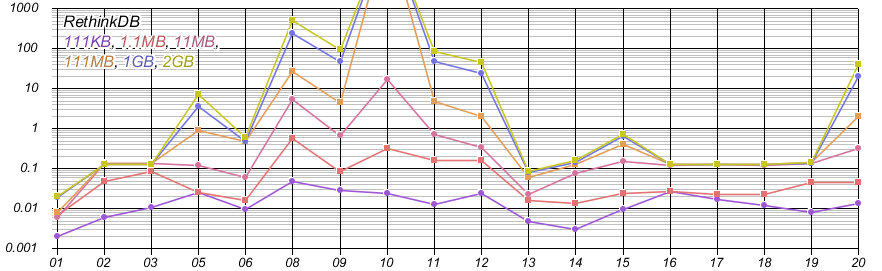
\includegraphics[width=0.95\textwidth]{img/result/rethinkdb/rethinkdb-all}
	\caption{XMark queries in RethinkDB}
	\label{fig:xmark-result-rethinkdb-all}
\end{figure}

\subsection{Couchbase}
Each Couchbase bucket is assigned RAM quota for caching data, therefore, the performance of a query depends on the amount of RAM allocated at the time of bucket creation. Figure~\ref{fig:xmark-result-cb-all} explains the query the performance of individual queries\todo{put all database images}. There were not any extraordinary phenomenon in Couchbase server.  Query Q1-Q3  were similar that of RethinkDB but Q5 and Q6 had produced comparatively better result due to its pre-defined reduce function \textit{\_count} in mapreduce. All the join queries were executed successfully in given time frame. Queries Q15-Q16 were performed slightly  better than that of other databases due to the JavaScript in map function. Another best result in Couchbase is aggregation query Q20, which is able to use pre-defined \textit{\_sum} in reduce part of Mapreduce. 

\begin{figure}
	\centering
	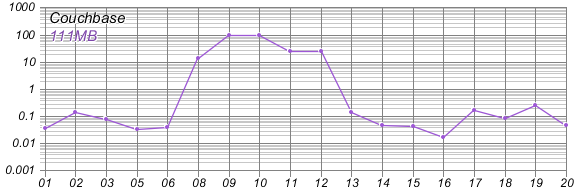
\includegraphics[width=0.95\textwidth]{img/result/cb/cb-all}
	\caption{XMark queries in Couchbase}
	\label{fig:xmark-result-cb-all}
\end{figure}

\subsection{Conclusion}
Even though our aim is not directly compare query performance in different systems, it would be interesting to see how these queries look like together. Figure~\ref{fig:xmark-result-1-all-new} illustrates all the queries for different database systems together for 111MB XMark data instance. MongoDB and BaseX have produced the best result in Q1. In Q2 and Q3, all database except MongoDB  had an identical result but in Q5 and Q6 MongoDB was the clear leader followed by Couchbae and BaseX, whereas RethinkDB was lagged behind other databases. In the join queries, the results produced by different databases were mixed in nature. MongoDB and BaseX were relatively better in Q8 and Q9 followed by Couchbase and RethinkDB. In Query Q10, the RethinkDB was failed to return result in given time frame but all other databases has identical results. The value join queries Q11 and Q12 were the best queries for RethinkDB followed by MongoDB and Couchbase but BaseX could not complete the result. Even the Q13 has similar results for all systems, RethinkDB had generated the best performance followed by MongoDB due to their efficient indexes. The FT search query Q14 is substring search for NoSQL databases, so that the query look little bit faster on them. The complex path queries Q15 and 16 Basex has better result with Couchbase than RethinkDB and MongoDB.
Q17-Q19 result are identical but in Q20 the Couchbase was the leader followed by Basex, MongoDB and RethinkDB. 
\\
\\
It has been seen that the NoSQL queries that were able to use secondary indexes performed better than BaseX with some exception. Even though some NoSQL do not support join queries, the result they produces are competitive in nature. The reason was favourable data model defined for those databases compare to BaseX and efficient read operation they produces. BaseX would probably perform better if the queries were optimized or data were normalized.  

\begin{table}[H]
\tiny
\begin{tabular}{|c|c|c|c|c|c|c|c|c|c|c| c|c|c|c|c|c|c|c|c|c|c|  } 
   db &  1 & 2 & 3 & 5 & 6  & 8 & 9 & 10  & 11 & 12 & 13 & 14 & 15 & 16 & 17 & 18 & 19 & 20 \\
 \hline
M\hbox{\pdfliteral{1 1 0 rg}\vrule height2mm width2mm depth0mm\pdfliteral{0 g}} & .00 & .75 & .78 & .01 & .00 & 1.17 & 1.65 & 87.25 & 23.13 & 7.21 & .05 & .55 & .20 & .17 & .11 & .22 & .11 & .21 \\
B\hbox{\pdfliteral{0 1 0 rg}\vrule height2mm width2mm depth0mm\pdfliteral{0 g}} & .04 & .19 & .17 & .10 & .19 & 2.31 & 2.43 & 89.36 & udf & udf & .36 & 1.23 & .08 & .08 & .15 & .36 & .52 & .19 \\
C\hbox{\pdfliteral{1 0 0 rg}\vrule height2mm width2mm depth0mm\pdfliteral{0 g}} & .04 & .14 & .08 & .03 & .04 & 13.2 & 98.1 & 94.1 & 24.1 & 26.1 & .13 & .05 & .04 & .02 & .17 & .09 & .27 & .05 \\
R\hbox{\pdfliteral{0 0 1 rg}\vrule height2mm width2mm depth0mm\pdfliteral{0 g}} & .01 & .14 & .14 & .94 & .68 & 26.76 & 4.53 & .00 & 4.80 & 2.10 & .02 & .18 & udf & .13 & .13 & .13 & .14 & 2.04 \\
\end{tabular}
\end{table}
\begin{figure}[H]
	\centering
	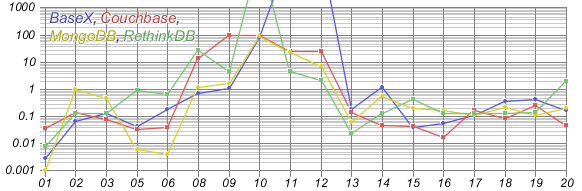
\includegraphics[width=0.85\textwidth]{img/result/1/1-all-new}
	\caption{XMark queries of 111MB data in all databases }
	\label{fig:xmark-result-1-all-new}
\end{figure}

























********** end here ******************


Figure~\ref{fig:xmark-result-basex-all} presents the time measuremnt of  XMark queries in BaseX. As mentioned earlier section, Q4 and Q7 are skipped because these queries cannot be translated into other NoSQL databases.  
	
We are using different charts for each of these databases instead of combine all the databases in a single chart. The queries are represented in x-axis with execution time in seconds is shown y-axis with limit 100 seconds. Queries Q4 and Q7 excluded in chart because they cannot be applied in NoSQL databases.


\begin{figure}[H]
	\centering
	\subfloat[BaseX]{
		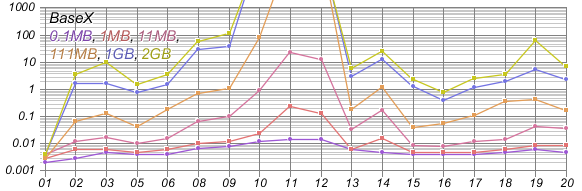
\includegraphics[width=0.95\textwidth]{img/result/basex/basex-all}
		\label{fig:xmark-result-1-basex}
	}\\
	
	\centering
	\subfloat[MongoDB]{
		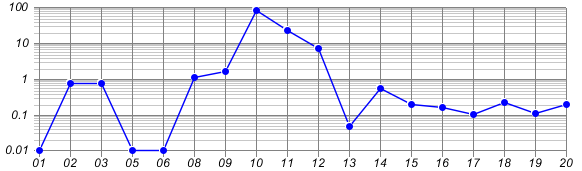
\includegraphics[width=.95\textwidth]{img/result/1/mongo}
		\label{fig:xmark-result-1-mongo}
	}\\
	
	\centering
	\subfloat[RethinkDB]{
		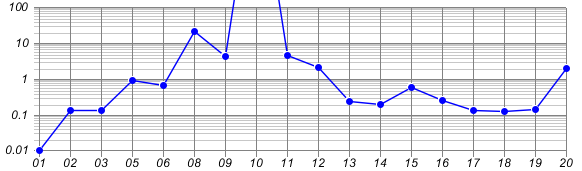
\includegraphics[width=.95\textwidth]{img/result/1/rethink}
		\label{fig:xmark-result-1-rethink}
	}\\
	
	\centering
	\subfloat[Couchbase]{
		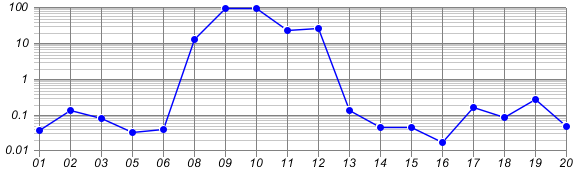
\includegraphics[width=.95\textwidth]{img/result/1/cb}
		\label{fig:xmark-result-1-cb}
	}
	
	
	\caption{Processing of XMark Queries on 111MB XMark instance}
	\label{fig:xmark-result-1-all}
\end{figure}
\begin{comment}
\begin{figure}[H]
	\centering
	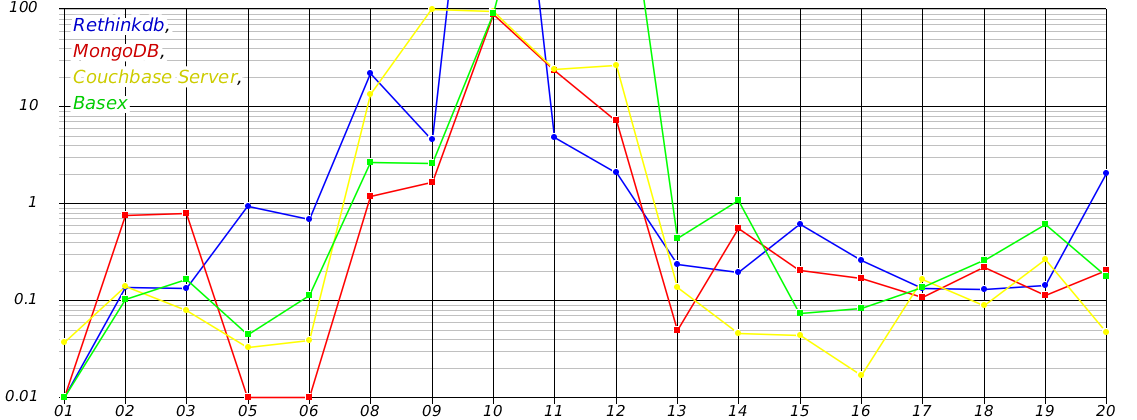
\includegraphics[width=1\textwidth]{img/result/1/all-2-2}
	\caption{Processing of Queries on 111MB XMark instance  in differet databases}
	\label{fig:xmark-result-all}
\end{figure}
\end{comment}


The result of individual queries will be explained here: 
 \begin{itemize}
 \item 
 The query Q1 is a simple query to handle string comparison. The whole query was evaluated  in less than 0.2mm in MongoDB followed by RethinkDB that has 0.6mm execution time while Couchbase needed 4mm. In MongoDB and RethinkDB, the comparison criteria was against primary index \textit{\_id} and \textit{id} respectively that improve the execution time significantly but Couchbase has to query through mapreduce with field filter that make query slow. BaseX executed query in less than 4mm.
 \item 
 Query Q2 and Q3 tests the positional operators. Couchbase offer the best performance followed by RethinDB, BaseX and Mongodb with big spike.In MongoDB, the aggregation pipeline with multiple stages reduces the performance of queries.
  \item 
  The MongoDB offer the best performance for the numerical comparison query Q5. A secondary index was created on attribute \textit{price} that boosted the performance. All the queries that uses count() function  are relatively slow in RethinkDB, the Q5 took also relatively longer time to return result than other databases. The Couchbase  is in second place with less than 4ms followed by BaseX almost 10ms execution time. 
  %6
  \item The query Q6 is once again produces best result in MongoDB. The count operation in a collection is relatively faster operation. The Couchbase also produces good result less than 5ms and BaseX around 10ms but RethinkDB is again slow due to count() function.
 % 8-9 
  \item The equi-join queries Q8 and Q9  are illustrated in Figure~\ref{fig:queries-8-9}. MongoDB has best performance in both queries with less than 2 seconds. The efficiency is improved due secondary indexes used in MongoDB. BaseX produces better result than Couchbase and RethinkDB with less than 3 seconds execution time.  Couchbase  was too slow to evaluate all join queries.
 %10
 \item The complex reconstruction query Q10 is one of most worst performing query for all database in average. A large output with various new fields are generated.  All databases took over 90 seconds to return the result. Basex,Couchbase and MongoDB evalueted in similar time but RethinkDB could not complete the query in time limit of 100 seconds 
 
 \item The value join queries  Q11 and Q12  two best queries for RethinkDB compare to other databases. The join between the tables supported by RethinkDB helps to evaluate the query relatively shorter time. BaseX could not complete these queries in specified time frame. As in Figure~\ref{fig:queries-11-12}, the MongoDB and couchbase have similar execution time for both query.
 \end{itemize}
 
 
\begin{figure}[H]
		\centering
		\subfloat[]{
			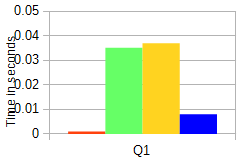
\includegraphics[width=0.3\textwidth]{img/result/1/11}
			%\caption{R-tree structure}
			\label{fig:queries-1}
		}
		\centering
		\subfloat[]{
			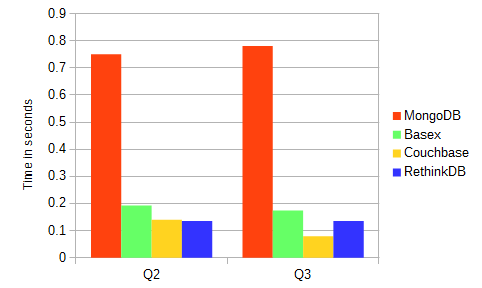
\includegraphics[width=0.6\textwidth]{img/result/1/2-3}
			%\caption{R-tree}
			\label{fig:queries-2-3}
		}\\
		\centering
		\subfloat[]{
			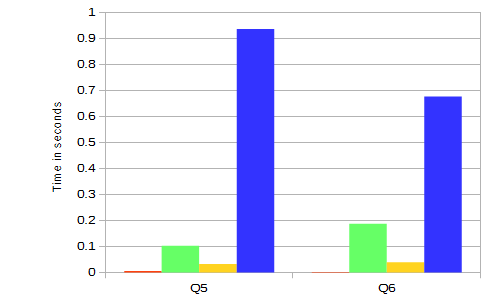
\includegraphics[width=0.5\textwidth]{img/result/1/5-6-2}
			%\caption{R-tree}
			\label{fig:queries-5-6}
		}
		\caption{XMark simple queries}
		\label{fig:query-result}
\end{figure}

 \begin{figure}[H]
		\centering
		\subfloat[]{
			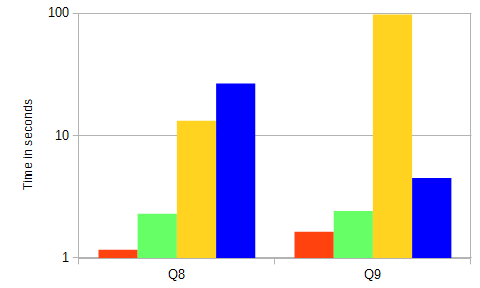
\includegraphics[width=0.5\textwidth]{img/result/1/join-queries-8-9}
			%\caption{R-tree}
			\label{fig:queries-8-9}
		}
		\centering
		\subfloat[]{
			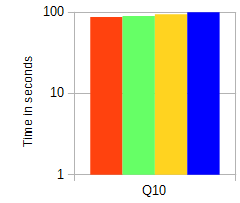
\includegraphics[width=0.3\textwidth]{img/result/1/join-queries-10}
			%\caption{R-tree}
			\label{fig:queries-10}
		}\\
		\centering
		\subfloat[]{
			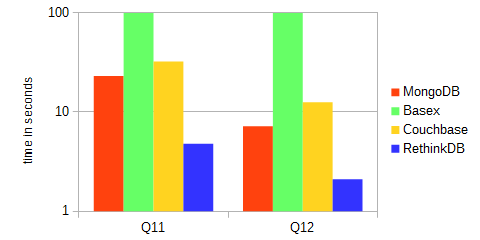
\includegraphics[width=0.8\textwidth]{img/result/1/join-queries-11-12}
			%\caption{R-tree}
			\label{fig:queries-11-12}
		}
		
		\caption{XMark Join Queries.}
		\label{fig:query-result-2}
	\end{figure}
	
\begin{figure}[H]
		\centering
		\subfloat[]{
			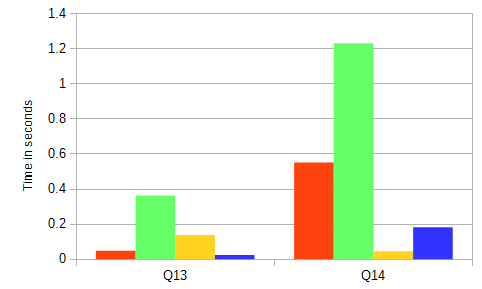
\includegraphics[width=0.4\textwidth]{img/result/1/13-14}
			%\caption{R-tree}
			\label{fig:queries-13-14}
		}
		\centering
		\subfloat[]{
			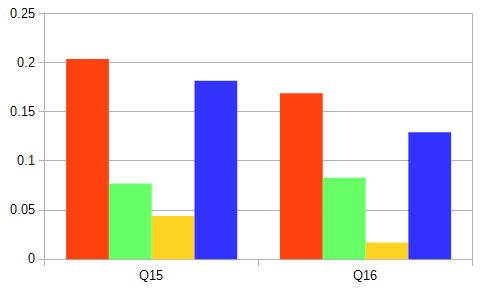
\includegraphics[width=0.4\textwidth]{img/result/1/15-16}
			%\caption{R-tree}
			\label{fig:queries-15-16}
		}\\
		\centering
		\subfloat[]{
			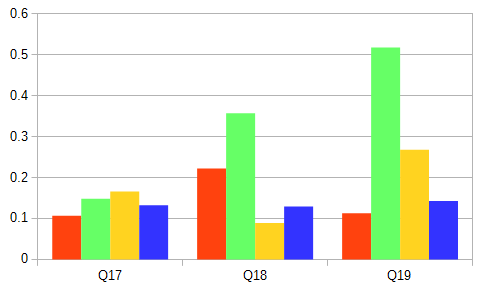
\includegraphics[width=0.5\textwidth]{img/result/1/17-18-19}
			%\caption{R-tree}
			\label{fig:queries-17-19}
		}
		\centering
		\subfloat[]{
			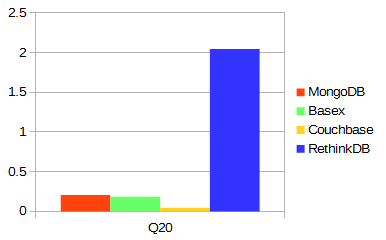
\includegraphics[width=0.4\textwidth]{img/result/1/20}
			%\caption{R-tree}
			\label{fig:queries-20}
		}
		\caption{XMark Advanced Queries.}
		\label{fig:query-result-3}
	\end{figure}
 
 \begin{comment}
  \begin{figure}[H]
		\centering
		\subfloat[XMark Queries No. 1 to 7]{
			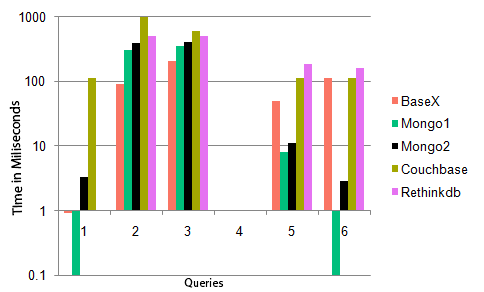
\includegraphics[width=0.3\textwidth]{img/result/1-6}
			%\caption{R-tree structure}
			\label{fig:queries-1-7}
		}
		\centering
		\subfloat[Join Queries (No. 8 to 12)]{
			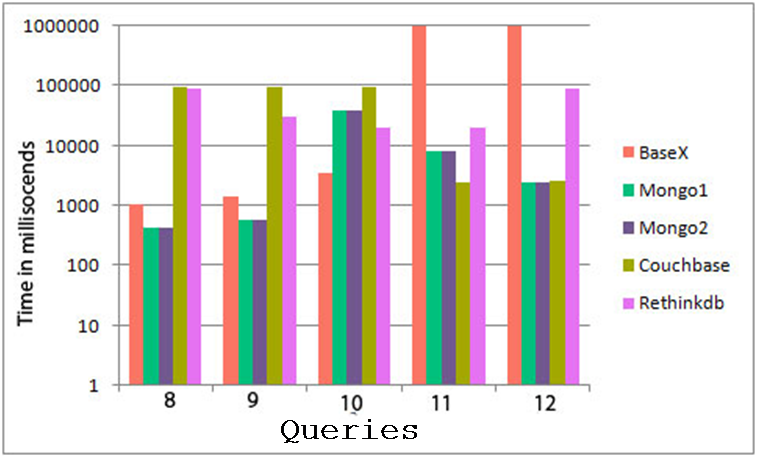
\includegraphics[width=0.5\textwidth]{img/result/8-12}
			%\caption{R-tree}
			\label{fig:queries-8-13}
		}
		
		\centering
		\subfloat[Queries 13 to 20]{
			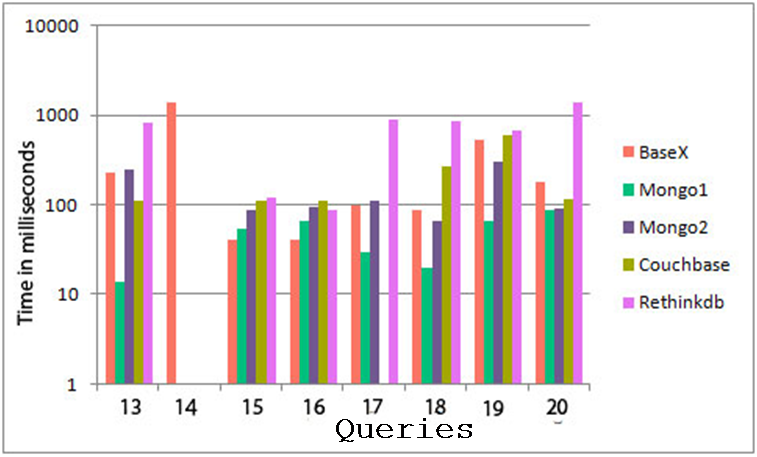
\includegraphics[width=0.44\textwidth]{img/result/13-20}
			%\caption{R-tree}
			\label{fig:queries-13-20}
		}
		\caption{XMark Queries time in XML and NoSQL databases(Mongo1: Mongodb shell, mongo2:through application)}
		\label{fig:query-result}
		
	\end{figure}
\end{comment}